\section{Suggestions to Improve the Existing System}

\subsection{System Perspective}

% Checked in grammarly
\afetbilgi\ is not part of a more extensive system. It is a standalone and open-source efforted website to verify critical information in the fight against the 6 February 2023 Pazarcik Earthquake and deliver it to disaster victims and those who want to help in an understandable, concise manner in multiple languages.

This information is presented in either the form of legible tables with third-party governmental and private links or an interactable method via a map view interface. If deemed necessary, admin and maintainers can make changes to display newly created or edited data and upload it to the system upon any complaints or suggestions they may get on their contact details.

\begin{figure}[H]
  \centering
  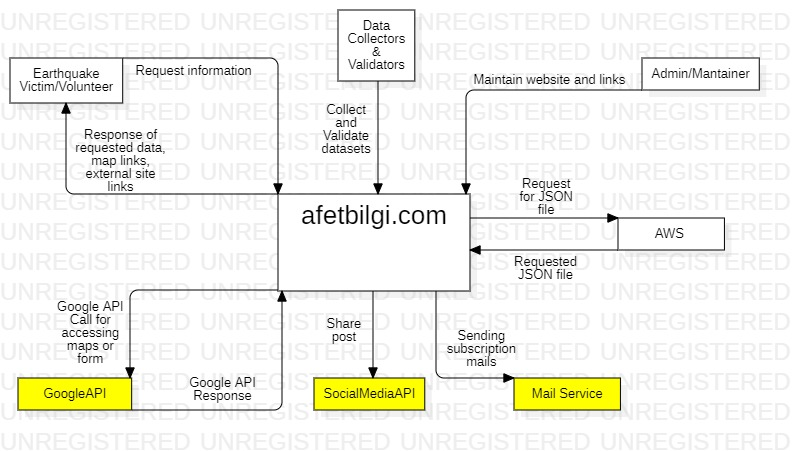
\includegraphics[width=\linewidth]{img/context-diagram-s4.jpg}
  \caption{Suggested New Context Diagram for \afetbilgi}
\end{figure}

\vfill
\newpage

The \afetbilgi\ consists of a combination of small physical and software parts. With the help of interfaces, these parts communicate among themselves and with the user. The following are the interfaces through which interaction occurs:
\begin{itemize}
  \setlength{\itemsep}{1pt}
  \item User interfaces
  \item Software interfaces
  \item Communication interfaces
\end{itemize}
Users interact with the website through their devices connected to the internet, such as cell phones or computers, as the user interface. The software interface enables the website to serve additional features to the user.

\subsubsection{User Interfaces}

In order to start using the website, a user should go into the website via a device connected to the internet. The website may have some loading time. After loading, the website is ready for user interactions. Users can interact with \afetbilgi\ directly to access required information.

The user interface contains \href{https://mui.com/}{MUI} components which are clear buttons and lists. Users can interact with the buttons to access the list of information or access more options related to the chosen information type.

\subsubsection{Software Interfaces}

\afetbilgi\ runs mainly JavaScript code with React library. It also uses additional react libraries such as \href{https://mui.com/}{MUI}.

The website makes necessary request to use some features such as accessing Google API, social media APIs and mail service.

\subsubsection{Communication Interfaces}

Since \afetbilgi\ is a website, it communicates via HTTPS (Hypertext Transfer Protocol Secure) and underlying protocols such as TCP/IP. It uses HTTPS to access APIs and servers.

\subsection{External Interfaces}

\vfill
\begin{figure}[H]
  \centering
  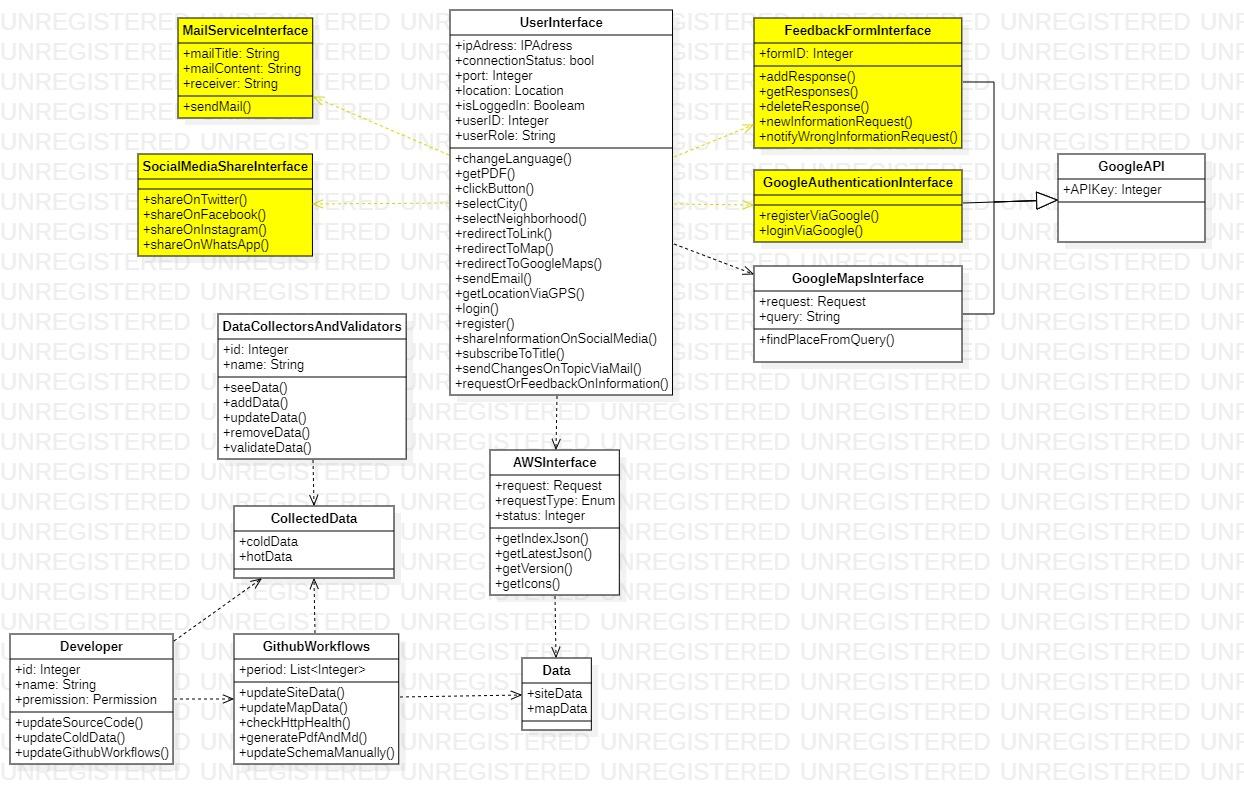
\includegraphics[width=\linewidth]{img/external-interfaces-s4.jpg}
  \caption{Suggested New External Interfaces}
\end{figure}
\vfill
\newpage

\subsection{Functions}

\vfill
\begin{figure}[H]
  \centering
  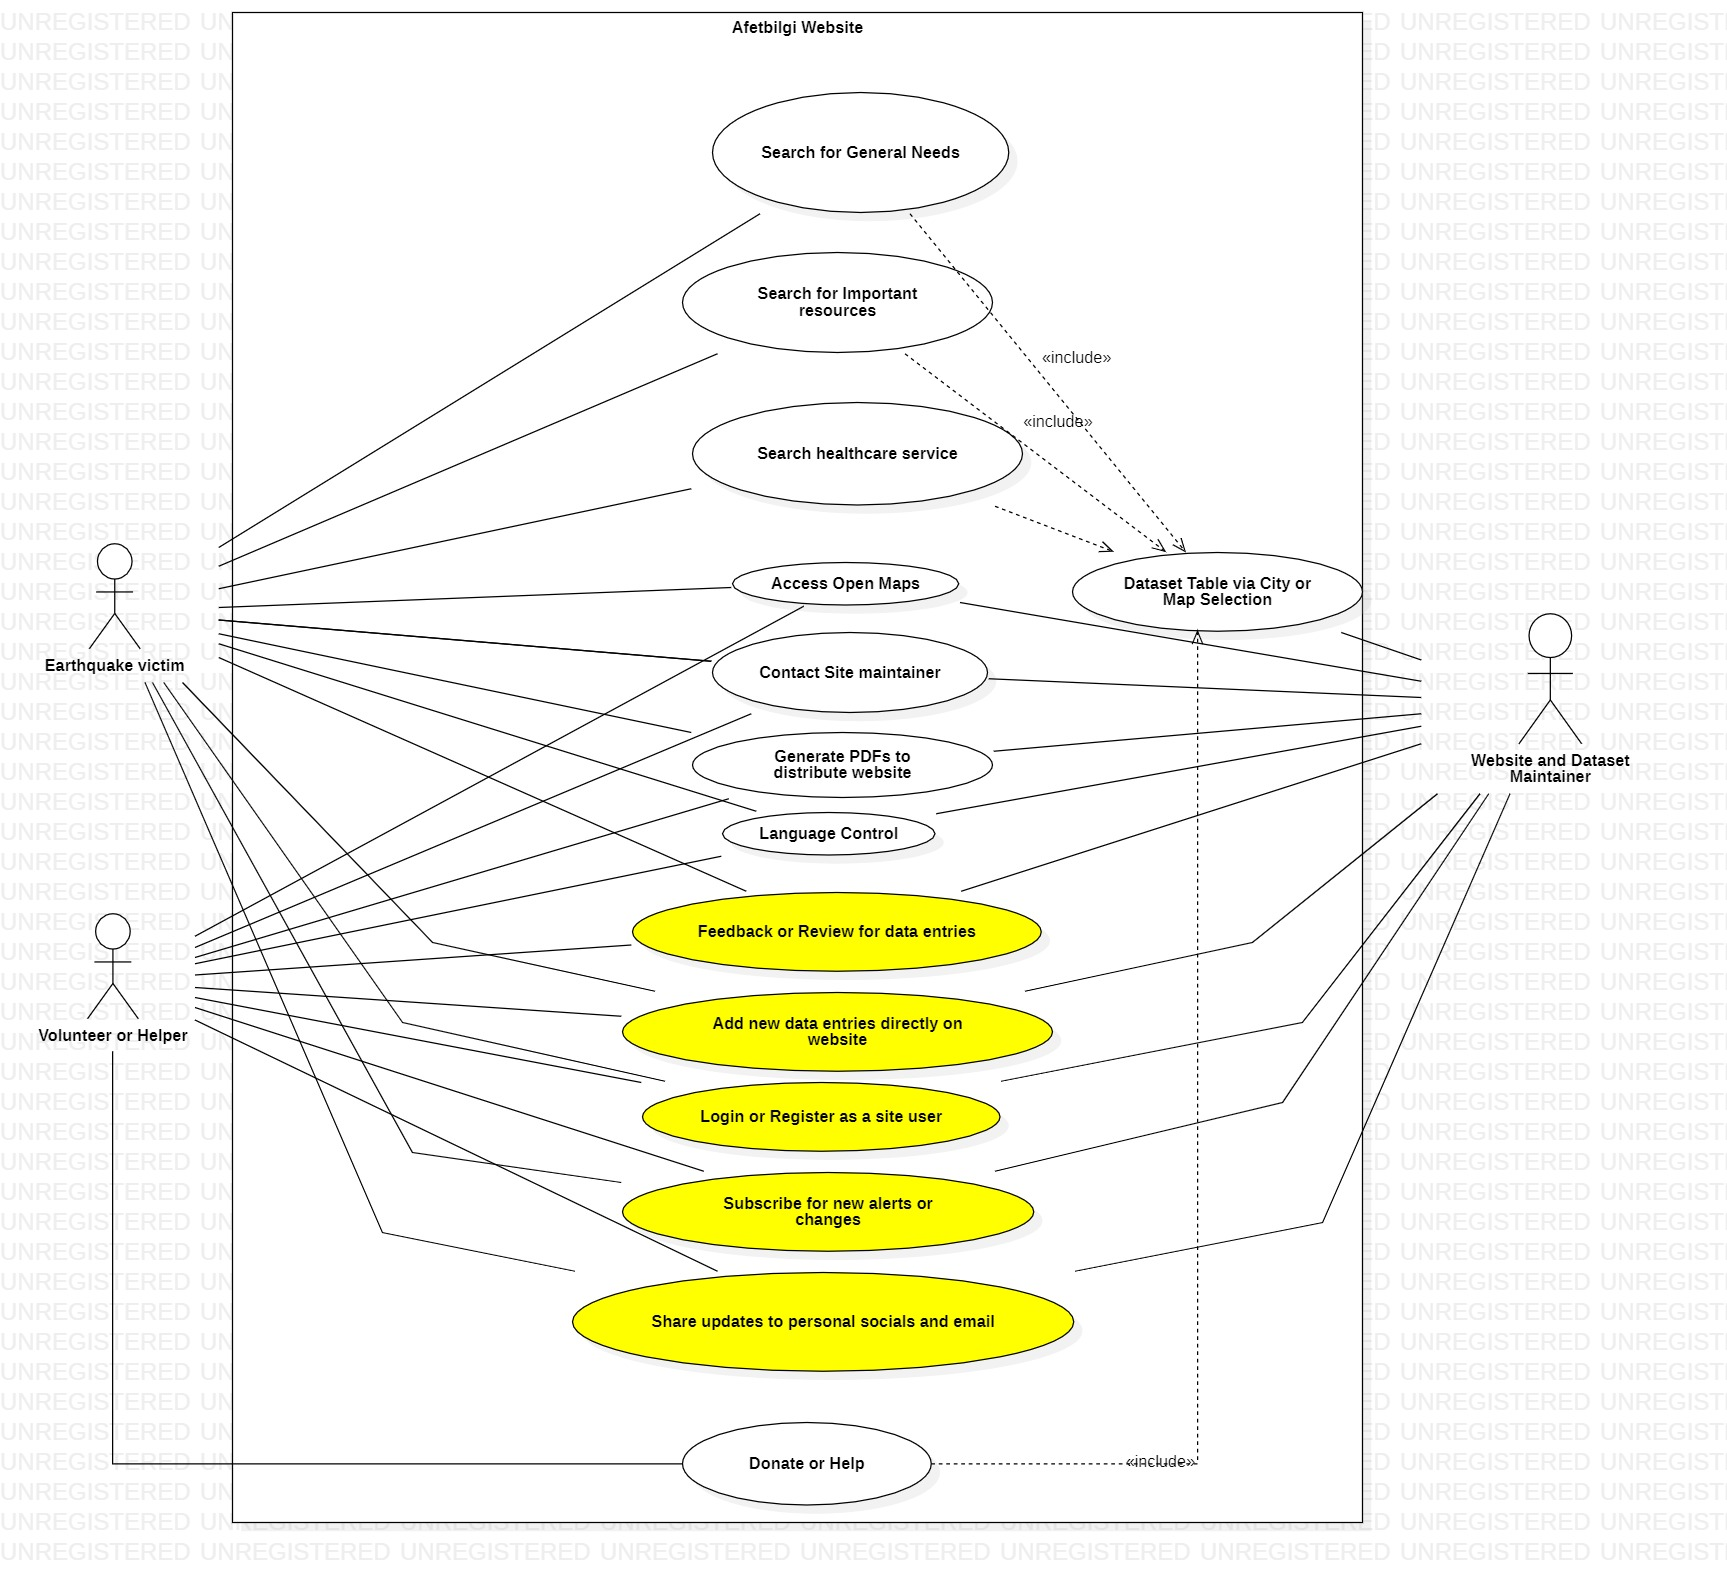
\includegraphics[width=\linewidth]{img/use-case-diagram-s4.jpg}
  \caption{Suggested New Use Case Diagram for \afetbilgi}
\end{figure}
\vfill
\newpage

% Feedback/Review for data entries
\begin{table}[H]
  \centering
  \refstepcounter{useCaseID}
  \resizebox{\linewidth}{!}{%
    \begin{tabular}{|p{.3\linewidth}|p{.7\linewidth}|}
      \hline
      \textbf{Use Case ID} & \theuseCaseID \\
      \hline
      \textbf{Use-Case Name} & Feedback/Review for data entries \\
      \hline
      \textbf{Actors} & Victims, Helpers and Site contributors \\
      \hline
      \textbf{Description} & Users can review existing data entries as per their usefulness, trustworthiness, and overall reception. Contributors can review and publish these changes. \\
      \hline
      \textbf{Data} & Form data \\
      \hline
      \textbf{Preconditions} & Preconditions	Users are to submit any proof/evidence of having used these facilities. \\
      \hline
      \textbf{Stimulus} & Logged in users can click on the review button next to a data entry in a table. \\
      \hline
      \textbf{Basic Flow} & 
        \begin{minipage}[H]{\linewidth} 
          \begin{enumerate}[label=\textbf{Step \arabic*:},leftmargin=1.5\leftmargin]
            \item User clicks on review button next to a data entry.
            \item User adds information such as any evidence of experience, written comments as well as rating on a fixed scale for usefulness.
            \item User submits the review form.
            \item Site contributor receives this in the realtime database employed.
            \item Report is approved and published onto website.
          \end{enumerate}
        \end{minipage} \\
      \hline
      \textbf{Alternative Flow \#1} & 
        \begin{minipage}[H]{\linewidth} 
          \begin{enumerate}[label=\textbf{Step \arabic*:},leftmargin=1.5\leftmargin]
            \item User clicks on review button next to a data entry.
            \item User adds information such as any evidence of experience, written comments as well as rating on a fixed scale for usefulness.
            \item User submits the review form.
            \item Site contributor receives this in the realtime database employed.
            \item Report is approved and published onto website.
            \item Report is unapproved and hence not published onto website.
          \end{enumerate}
        \end{minipage} \\
      \hline
      \textbf{Alternative Flow \#2} & - \\
      \hline
      \textbf{Exception Flow} & - \\
      \hline
      \textbf{Post Conditions} & User report is either published if approved or not published if unapproved. \\
      \hline
    \end{tabular}
  }
  \caption{Use Case - Feedback/Review for data entries}
\end{table}

% State Diagram - Feedback/Review for data entries
\begin{figure}[H]
  \centering
  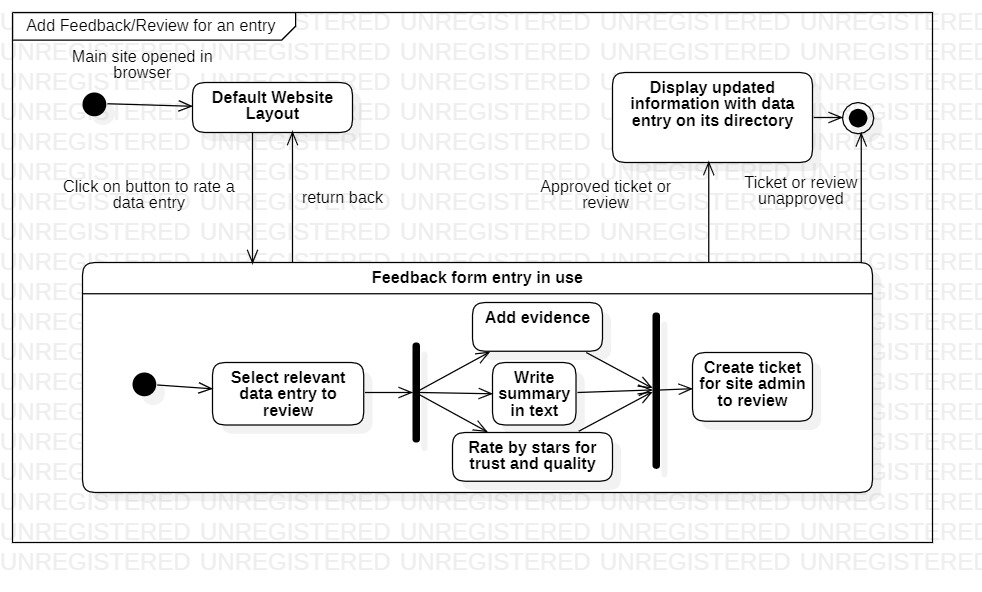
\includegraphics[width=\linewidth]{img/state-diagram-s4-feedback-review.jpg}
  \caption{State Diagram - Feedback/Review for data entries}
\end{figure}

% Add new data entries directly onto website
\begin{table}[H]
  \centering
  \refstepcounter{useCaseID}
  \resizebox{\linewidth}{!}{%
    \begin{tabular}{|p{.3\linewidth}|p{.7\linewidth}|}
      \hline
      \textbf{Use Case ID} & \theuseCaseID \\
      \hline
      \textbf{Use-Case Name} & Add new data entries directly onto website \\
      \hline
      \textbf{Actors} & Victims, Helpers and Site contributors \\
      \hline
      \textbf{Description} & Users can add new data entries as per their usefulness, trustworthiness, and overall reception in their relevant category. \\
      \hline
      \textbf{Data} & Form data \\
      \hline
      \textbf{Preconditions} & Users can submit any proof/evidence of having used these facilities. \\
      \hline
      \textbf{Stimulus} & Logged in users can click on the add button next to a category type. \\
      \hline
      \textbf{Basic Flow} & 
        \begin{minipage}[H]{\linewidth} 
          \begin{enumerate}[label=\textbf{Step \arabic*:},leftmargin=1.5\leftmargin]
            \item User clicks on add button next to a category entry.
            \item User adds information such as any evidence of experience, written comments as well as rating on a fixed scale for usefulness.
            \item User submits the add new data entry form.
            \item Site contributor receives this in the realtime database.
            \item Report is approved and hence a new data entry is published onto website.
          \end{enumerate}
        \end{minipage} \\
      \hline
      \textbf{Alternative Flow \#1} & 
        \begin{minipage}[H]{\linewidth} 
          \begin{enumerate}[label=\textbf{Step \arabic*:},leftmargin=1.5\leftmargin]
            \item User clicks on add button next to a category entry.
            \item User adds information such as any evidence of experience, written comments as well as rating on a fixed scale for usefulness.
            \item User submits the add new data entry form.
            \item Site contributor receives this in the realtime database.
            \item Report is unapproved and hence not published onto website.
          \end{enumerate}
        \end{minipage} \\
      \hline
      \textbf{Alternative Flow \#2} & - \\
      \hline
      \textbf{Exception Flow} & - \\
      \hline
      \textbf{Post Conditions} & User's new recommendation is either published if approved or not published if unapproved. \\
      \hline
    \end{tabular}
  }
  \caption{Use Case - Add new data entries directly onto website}
\end{table}

% Activity Diagram - Add new data entries directly onto website
\begin{figure}[H]
  \centering
  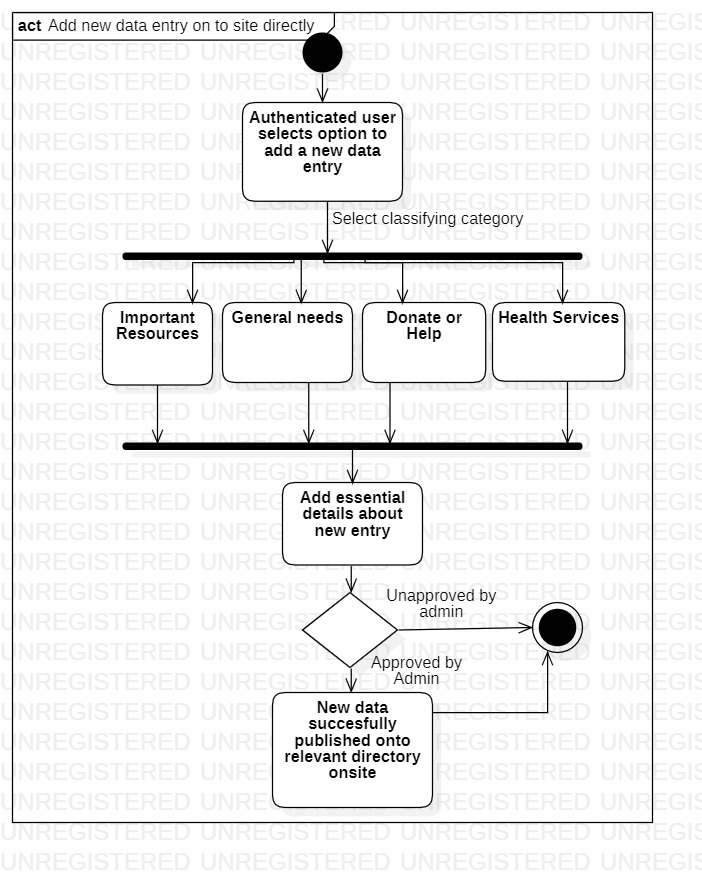
\includegraphics[width=\linewidth]{img/activity-diagram-s4-add-new-data.jpg}
  \caption{Activity Diagram - Add new data entries directly onto website}
\end{figure}

% User can Login/Register themselves
\begin{table}[H]
  \centering
  \refstepcounter{useCaseID}
  \resizebox{\linewidth}{!}{%
    \begin{tabular}{|p{.3\linewidth}|p{.7\linewidth}|}
      \hline
      \textbf{Use Case ID} & \theuseCaseID \\
      \hline
      \textbf{Use-Case Name} & User can Login/Register themselves \\
      \hline
      \textbf{Actors} & Users: Victims or Helpers \\
      \hline
      \textbf{Description} & Users can register themselves to allow an appreciable level of authenticated trust in the website's recommendations. \\
      \hline
      \textbf{Data} & Form data containing sensitive information and credentials \\
      \hline
      \textbf{Preconditions} & Users have to submit a means of communication such as a phone number or email. \\
      \hline
      \textbf{Stimulus} & Website main page layout has a navigation bar that has an optional sign up/login button. \\
      \hline
      \textbf{Basic Flow} & 
        \begin{minipage}[H]{\linewidth} 
          \begin{enumerate}[label=\textbf{Step \arabic*:},leftmargin=1.5\leftmargin]
            \item User clicks on the register button in the top navigation bar.
            \item User add details such a account name, phone number and so on in the form. Phone number/email entered is verified by an AWS IAM service.
            \item User creates an authenticated account onto the site.
          \end{enumerate}
        \end{minipage} \\
      \hline
      \textbf{Alternative Flow \#1} & 
        \begin{minipage}[H]{\linewidth}
          \begin{enumerate}[label=\textbf{Step \arabic*:},leftmargin=1.5\leftmargin]
            \setcounter{enumi}{1}
            \item User use Google Register option. Authentication is checked and verified by Google Authentication API.
            \item User creates an authenticated account onto the site.
          \end{enumerate}
        \end{minipage} \\
      \hline
      \textbf{Alternative Flow \#2} & 
        \begin{minipage}[H]{\linewidth} 
          \begin{enumerate}[label=\textbf{Step \arabic*:},leftmargin=1.5\leftmargin]
            \item User clicks on the login button in the top navigation bar.
            \item User adds his/her credentials such as email and password.
            \item Backend IAM service verifies and accepts.
            \item User is logged in.
          \end{enumerate}
        \end{minipage} \\
      \hline
      \textbf{Exception Flow} & 
        \begin{minipage}[H]{\linewidth}
          \begin{enumerate}[label=\textbf{Step \arabic*:},leftmargin=1.5\leftmargin]
            \setcounter{enumi}{2}
            \item Backend IAM service cannot verify and does not accept new user/log in credentials of user
            \item User adds his/her credentials such as email and password.
            \item User returned to previous mainpage.
          \end{enumerate}
        \end{minipage}
       \\
      \hline
      \textbf{Post Conditions} & User account is accessed and now allows to make active contributions to the site with reviews and recommendations. They receive account notifications on their email as well. \\
      \hline
    \end{tabular}
  }
  \caption{Use Case - User can Login/Register themselves}
\end{table}

% Sequence Diagram - User can Login/Register themselves
\begin{figure}[H]
  \centering
  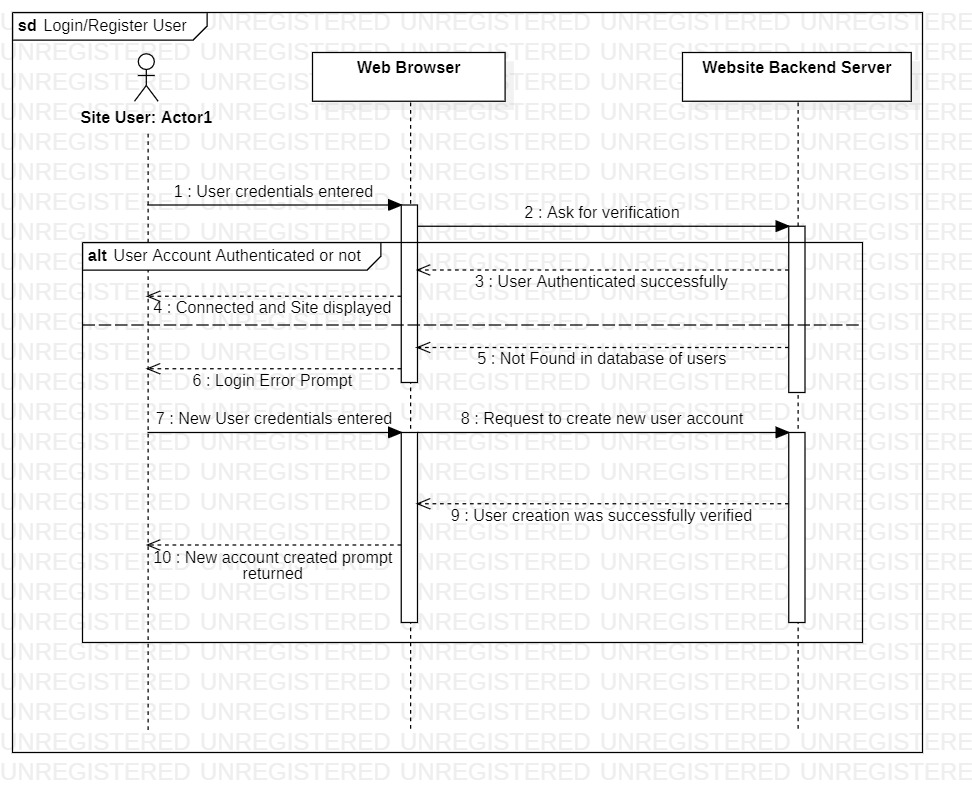
\includegraphics[width=\linewidth]{img/sequence-diagram-s4-login-register.jpg}
  \caption{Sequence Diagram - User can Login/Register themselves}
\end{figure}

\vspace*{\fill}
\newpage

% Users can subscribe to email/phone number for alerts
\begin{table}[H]
  \centering
  \refstepcounter{useCaseID}
  \resizebox{\linewidth}{!}{%
    \begin{tabular}{|p{.3\linewidth}|p{.7\linewidth}|}
      \hline
      \textbf{Use Case ID} & \theuseCaseID \\
      \hline
      \textbf{Use-Case Name} & Users can subscribe to email/phone number for alerts \\
      \hline
      \textbf{Actors} & Users: Victims or Helpers \\
      \hline
      \textbf{Description} & Users can receive new alerts/updates with regards to data. \\
      \hline
      \textbf{Data} & Email/Phone number of user (sensitive data). \\
      \hline
      \textbf{Preconditions} & Any of the above means of information communication must be chosen and entered. \\
      \hline
      \textbf{Stimulus} & User clicks on the Subscribe button on the navigation bar at the top. \\
      \hline
      \textbf{Basic Flow} & 
        \begin{minipage}[H]{\linewidth} 
          \begin{enumerate}[label=\textbf{Step \arabic*:},leftmargin=1.5\leftmargin]
            \item User clicks on the Subscribe button.
            \item User enters email/phone number.
            \item User selects topic(s) to get notified.
            \item User clicks on submit.
          \end{enumerate}
        \end{minipage} \\
      \hline
      \textbf{Alternative Flow \#1} & 
        \begin{minipage}[H]{\linewidth}
          \begin{enumerate}[label=\textbf{Step \arabic*:},leftmargin=1.5\leftmargin]
            \setcounter{enumi}{2}
            \item User clicks on unsubscribe.
            \item User selects the topic(s) to unsubscribe.
          \end{enumerate}
        \end{minipage} \\
      \hline
      \textbf{Alternative Flow \#2} & - \\
      \hline
      \textbf{Exception Flow} & - \\
      \hline
      \textbf{Post Conditions} & Users can now receive updates and similar notifications on their phone/email account. \\
      \hline
    \end{tabular}
  }
  \caption{Use Case - Users can subscribe to email/phone number for alerts}
\end{table}

% Users can share updates to their personal socials
\begin{table}[H]
  \centering
  \refstepcounter{useCaseID}
  \resizebox{\linewidth}{!}{%
    \begin{tabular}{|p{.3\linewidth}|p{.7\linewidth}|}
      \hline
      \textbf{Use Case ID} & \theuseCaseID \\
      \hline
      \textbf{Use-Case Name} & Users can share updates to their personal socials \\
      \hline
      \textbf{Actors} & Users: Victims/Helpers \\
      \hline
      \textbf{Description} & Users can share data/category onto their social media. \\
      \hline
      \textbf{Data} & User account permission data along with data entry from site data \\
      \hline
      \textbf{Preconditions} & Any of the above means of social media must be chosen and their account details entered. \\
      \hline
      \textbf{Stimulus} & Logged in users can click on the add button next to a data entry/category type. \\
      \hline
      \textbf{Basic Flow} & 
        \begin{minipage}[H]{\linewidth} 
          \begin{enumerate}[label=\textbf{Step \arabic*:},leftmargin=1.5\leftmargin]
            \item Use clicks on share button next to a category/data entry
            \item User is led to a pre created template onto the social media platform of their choice such as a Tweet for Twitter or Story for Instagram.
            \item User can edit/submit the template.
            \item User successfully shared this onto the selected platform.
          \end{enumerate}
        \end{minipage} \\
      \hline
      \textbf{Alternative Flow \#1} & - \\
      \hline
      \textbf{Alternative Flow \#2} & - \\
      \hline
      \textbf{Exception Flow} & - \\
      \hline
      \textbf{Post Conditions} & User has now shared the website and the concerned category type/data entry to the public/close relvatives. \\
      \hline
    \end{tabular}
  }
  \caption{Use Case - Users can share updates to their personal socials}
\end{table}

\vspace*{\fill}
\newpage

\subsection{Usability Requirements}

% Checked in grammarly
\begin{itemize}
  \item Users shall be able to register for the website with proper verification to avoid while also avoiding any potential discrimination.
  \item Users shall be able to add their identity details as they see fit while upholding their privacy and verifying their accounts for site maintainers to approve.
  \item Site maintainers shall allow users to prioritize alerts as per their subscription settings.
  \item Any new entries or reviews of existing entries shall have tickets reviewed before being approved for publication on the website.
\end{itemize}

\subsection{Performance Requirements}

% Checked in grammarly
\begin{itemize}
  \item \textbf{Privacy:} User account information has to be verified and safeguarded with a capable authentication service inclusive of AWS's IAM (Identity and Access Management) service.
  Security: Accounts must be verified with proper mechanisms such as sms and email verification to avoid scams/frauds.
  \item \textbf{Scalability:} Tickets for new data entries or reviews for existing ones must be reviewed fast by the site's team employing our proposed relational database system to track ticket ids and classify them as approved or not.
  \item \textbf{Social Media Integration:} Sharing data entries to external social media apps shall have prepared to post templates to save time(such as a Story template for Facebook and Instagram).
  \item \textbf{Accurate and current information:} \afetbilgi\ makes a new attempt to offer the best data entries, which have now been reviewed under a new scale of trust by users who can evaluate/offer feedback for entries.
\end{itemize}

\subsection{Logical Database Requirements}

\afetbilgi\ does currently have a relational database. To make minor difference in the source code, the object structure in the Section 3.5 is preserved. Additionally, users, roles and mail subscription data are added into database. \texttt{Users} relation provides information related to the login system. \texttt{Roles} relation provides information related to the registered role. \texttt{Mail Subscription} relation provides the information related to topics that users subcribed. \texttt{SiteInformation} relation provides information related to the information located in the website.

\begin{figure}[H]
  \centering
  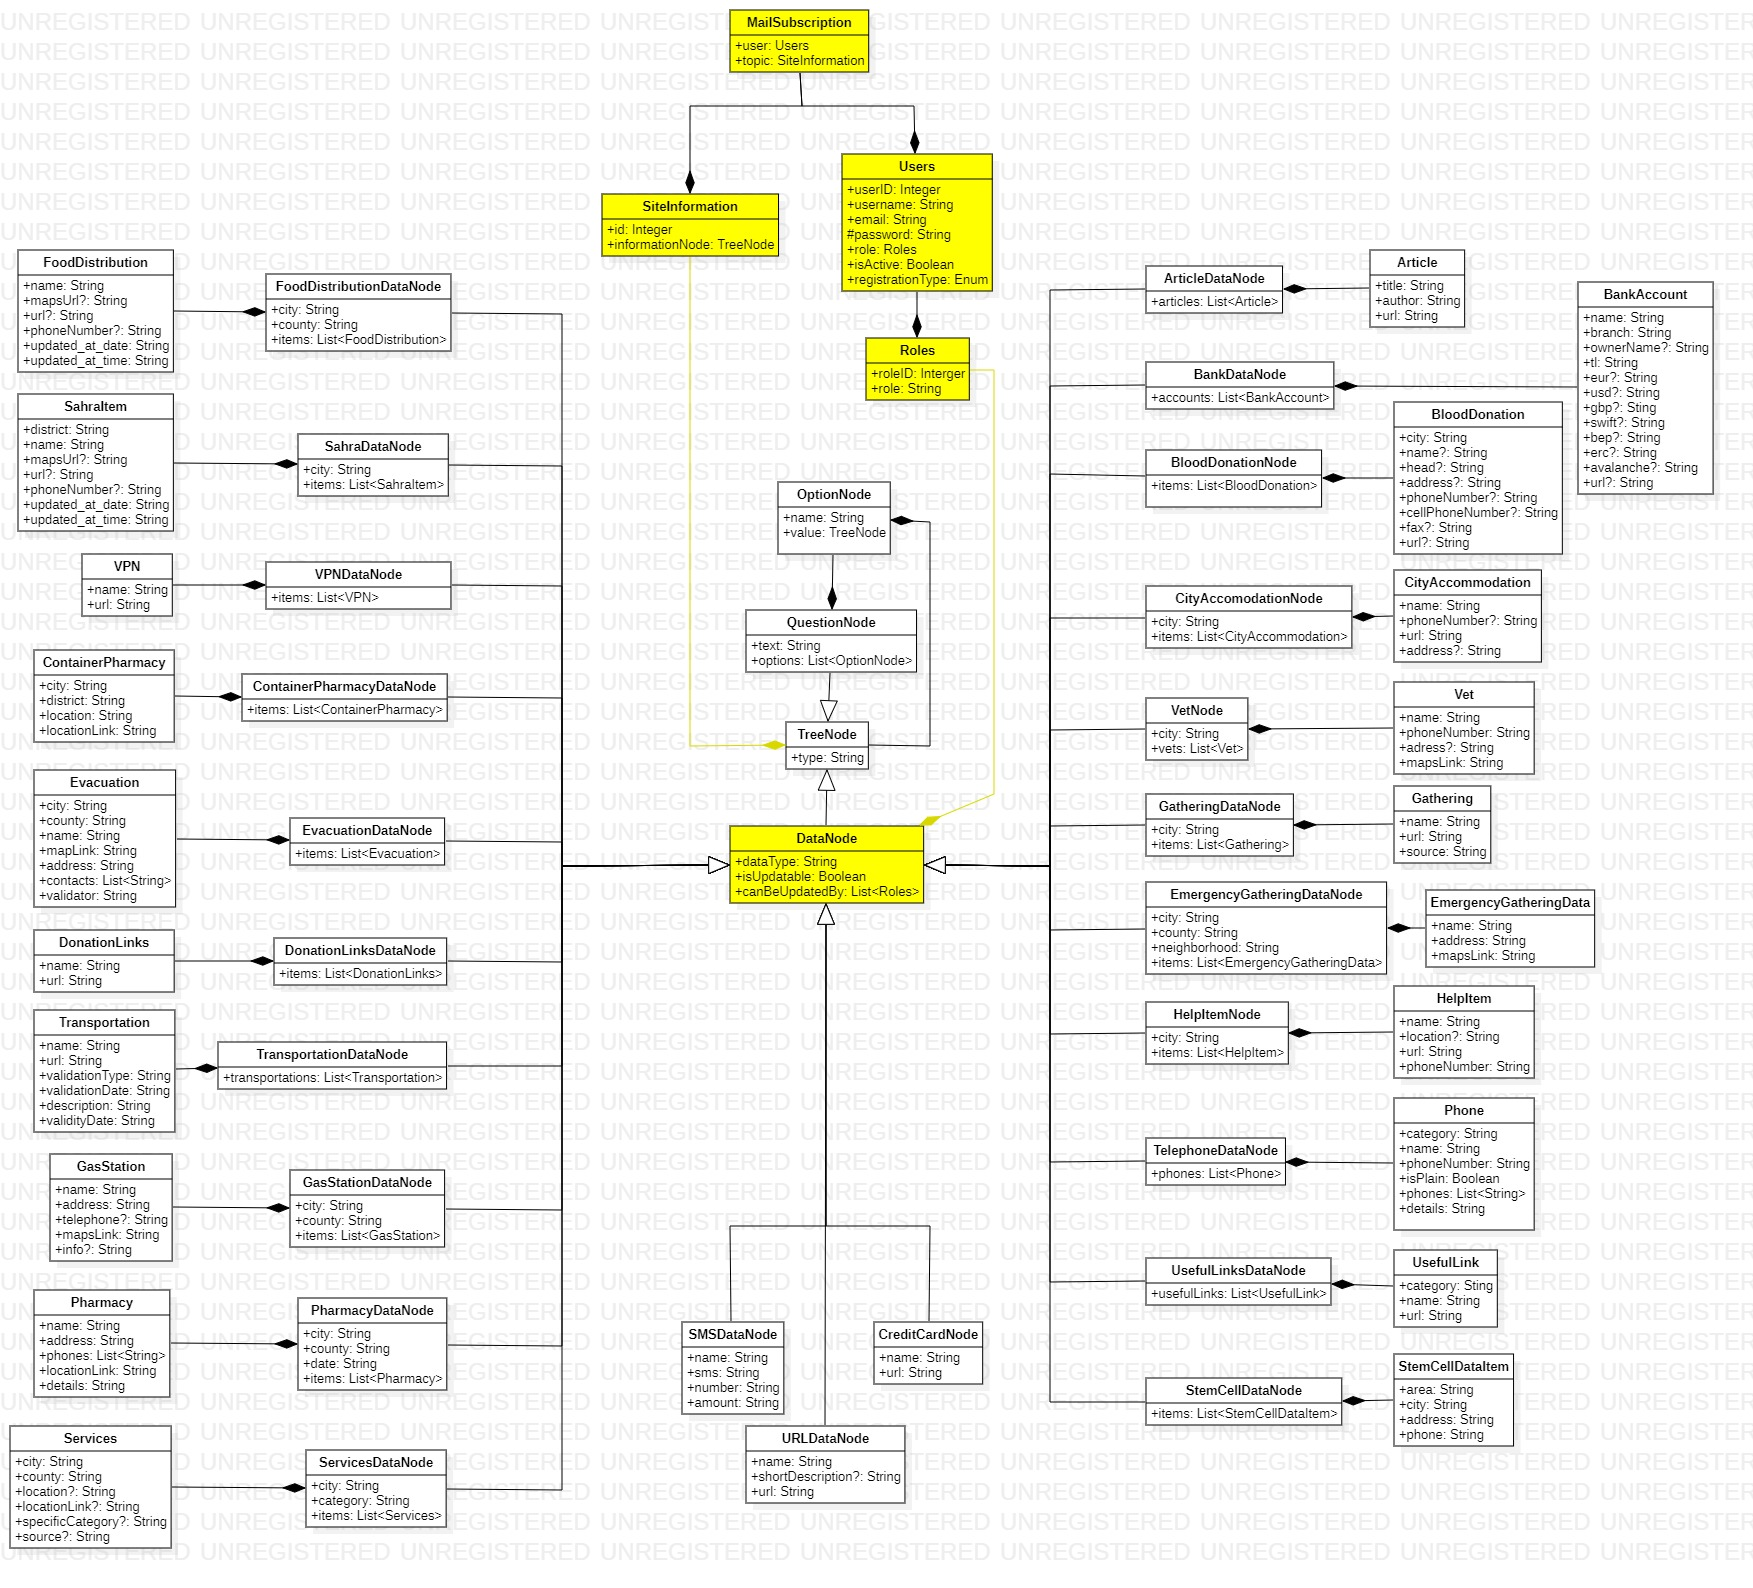
\includegraphics[width=\linewidth]{img/database-s4.jpg}
  \caption{Suggested New Relational Database}
\end{figure}

\subsection{Design Constraints}

% Checked in grammarly
The new features of afetbilgi do need more processing times from users, especially those requiring immediate information in a tense, urgent situation such as regarding a nearby hospital. 

With that in mind, additional improvements such Login/Register procedure could be made optional in case of simply reading data without any input from the user in the form of feedback for current data entries and adding input for new ones. On the other hand, though, improving communication in the form of sharing directly to personal socials and attaining email alerts for updates is also crucial to help users spread reliable intel fast and securely.

\subsection{System Attributes}

% Checked in grammarly
\begin{itemize}
  \item \textbf{Reliability:}
    \begin{itemize}[label=$\blacksquare$]
      \item A new open-source license (quoted in the repositories’ manual) would allow for more fair use by future contributors reliably.
      \item A more concretely established regulation policy and other plain Github workflows would help in continuous integration and development while keeping website health at best, such as via Jenkins/DevOps mechanisms integration.
      \item An audit mechanism has been introduced that allows the website entries to be viewed by human personnel in addition to automated Github workflows.
      \item Newly added feedback/data entries must be checked with human contributors to make them sensible and correspond to established data node interface conventions.
    \end{itemize}

  \vspace*{\fill}
  \newpage

  \item \textbf{Security and Privacy:}
    \begin{itemize}[label=$\blacksquare$]
      \item The login and Registration service ensures that users are verified before they can contribute to the website.
    \end{itemize}
  \item \textbf{Portability:}
    \begin{itemize}[label=$\blacksquare$]
      \item Users can share on their socials and even receive email and alerts via subscription to the website.
    \end{itemize}
\end{itemize}

\subsection{Supporting Information}

% Checked in grammarly
The website can be kept life for a couple of years or indefinitely with permanent government funding if needed by at least the Turkish government's own AFAD (disaster management) authority.

Precious information such as user details/data entries will always be protected under privacy laws under this supported website agreement with the government until site maintainers retire the site. 
